% \note{siehe woot}\\
\gls{OT} ist eine weit verbreitete Technik zur Unterstützung von Funktionalitäten in \gls{kollaborativ}er Software.
Sie stammt aus einer im Jahre 1989 veröffentlichten Forschungsarbeit und wurde ursprünglich nur für die gemeinsame Bearbeitung von Klartext-Dokumenten entwickelt~\cite{ot_paper}.
Heute unterstützt \gls{OT} zusätzlich das \gls{kollaborativ}e Bearbeiten von \gls{HTML}, RTF und XML Dokumenten, Adobe Flash\footnote{ Browserplugin, steht unter \url{https://get.adobe.com/de/flashplayer/} zum Download bereit} Grafiken und Dokumenten in CAD\footnote{ CAD, engl.: computer-aided design, deutsch: rechnerunterstütztes Konstruieren} Tools wie Autodesk Maya\footnote{ 3D Design Software. steht unter \url{https://www.autodesk.com/products/maya/free-trial} zum Download bereit}.
Des Weiteren können mit \gls{OT} Dateien die in Microsoft Office\footnote{ Bürosoftware, steht unter \url{https://products.office.com/de-de/compare-all-microsoft-office-products?tab=1} zum Download bereit} enthalten sind wie Word Dokumente, PowerPoint Folien und Excel Tabellen kollaborativ bearbeitet werden, aber auch Dokumente in webbasierte Anwendungen wie Google Docs\footnote{ Webanwendung, mit der Dokumente erstellt und kollaborativ bearbeitet werden können, \url{https://docs.google.com}} und Google Wave\footnote{ Google Wave war eine von Google vorgestelle Webanwendung zur Kommunikation und kollaborativer Zusammenarbeit}~\cite{ot-faq}.\\\\
%
%
Operational Transform ist ein Algorithmus für die Transformationen von Operationen, die auf Dokumente mit unterschiedlichen Zustand angewendet werden, um diese Dokumente in den identischen Zustand zu versetzen.
Jede Änderung an einem freigegebenen Dokument wird als Operation dargestellt.
Eine Operation ist die Repräsentation einer Änderung an einem Dokument und zeichnet im Wesentlichen den Unterschied zwischen einer und der nachfolgenden Version eines Dokuments auf.
Die Anwendung einer Operation auf das aktuelle Dokument führt zu einem neuen Dokumentstatus.
Es gibt beispielsweise die Operation \it{Einfügen}. 
Das Einfügen besteht aus dem eingefügten Text und dessen Position im Dokument. Die Operation die beschreibt 'Füge den Buchstaben x an dritter Stelle im Dokument ein' sieht so aus: (\tt{insert('x', 3)}).
Für die Position kann ein Koordinatensystem ermittelt werden, Zeilennummer und die Position in einer Zeile, oder das Dokument wie eine Folge von Zeichen behandeln werden.\\
%
\Gls{kollaborativ}e Systeme, die \gls{OT} verwenden, benutzen normalerweise den replizierten Dokumentenspeicher.
Das heißt auf jedem Gerät befindet sich eine eigene Kopie des Dokuments.
Die Operationen erfolgen auf der lokalen Kopie und die Änderungen werden an alle anderen Geräte weitergegeben.\\
Um gleichzeitige Operationen zu behandeln, gibt es eine Funktion (\tt{Transform} genannt), die zwei Operationen übernimmt, die auf denselben Dokumentstatus angewendet wurden (aber auf verschiedenen Clients).
Wenn ein Client die Änderungen von einem anderen empfängt, werden die Änderungen vor ihrer Ausführung transformiert~\cite{ot_paper}.\\
Daraus wird eine neue Operation berechnet, die nach der zweiten Operation angewendet werden kann.
Diese behält die erste beabsichtigte Änderung der Operation.\\
%
\clearpage
Die Grundidee des \gls{OT} Algorithmusses wird anhand eines Beispiels, das die \autoref{fig:ot} veranschaulicht, illustriert.\\
Es gibt den initialen Text ''abc'', der auf den Geräten der kollaborativ arbeitenden Personen, Amilia und Rory, besteht.
Amilia fügt lokal vor dem ''abc'' ein ''x'' ein, Rory löscht auf ihrem Gerät den Buchstaben ''c'''.
%
\begin{figure}[H]
  \centering
  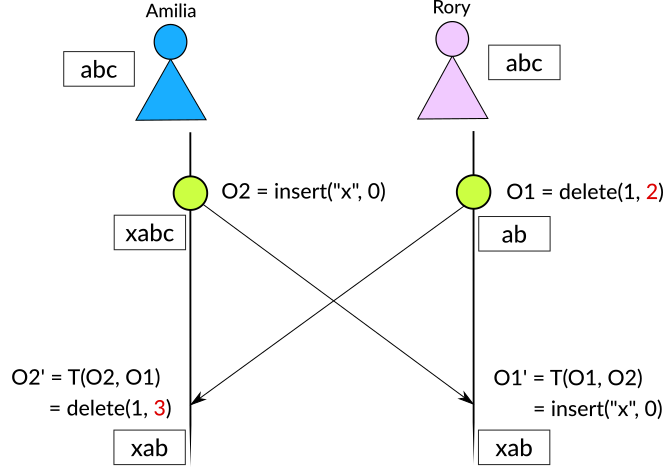
\includegraphics[width=0.8\textwidth]{ot-j}
  \grayRule
  \caption{Die Grundidee von \gls{OT}}
  \label{fig:ot}
\end{figure}
%
Die konkurrierenden Operationen sind \tt{insert(0, ''x'')}, 'Füge das Zeichen ''x'' an Stelle Null ein', und \tt{delete(2, 1)}, 'lösche ein Zeichen an der zweiten Stelle'.
In \gls{OT} werden lokale Änderungen angewandt, so wie sie passieren. Operationen über das Netzwerk werden, bevor sie auf zuvor ausgeführte Operationen angewandt werden, transformiert.\\
%
Wenn die Operation von Rory an Amilia gesendet und dort angewandt werden würde, gäbe es kein Problem. Der Buchstabe an zweiter Stelle wird gelöscht und danach wird an Stelle Null ein ''x'' eingefügt. Das Ergebis ist das gewünschte ''xab''.
Jedoch wenn die Operation von Amilia an Rory gesendet und dort angewandt werden würde, gäbe es eins. Dann würde der Buchstabe "b" gelöscht, da er sich, nachdem das ''x'' eingefügt wurde, an zweiter Stelle steht. Das Ergebnis nach der ersten Operation wäre ''xac''. Die Dokumentenstatus sind nicht identisch.\\
%
Wird die Operation \tt{delete(1, 2)} gegen die Operation von Amilia transformiert, wird berücksichtigt, dass Amilia ein Zeichen vor der Position zwei eingefügt hat.\\\\

Zuammenfassend besteht die Grundidee von \gls{OT} darin, 
durch die Transformationen


die Parameter einer Operation gemäß den Auswirkungen \b{zuvor ausgeführter} konkurrierender Operationen anzupassen, so dass die transformierte Operation die korrekte Wirkung erzielen und die Dokumentenkonsistenz aufrechterhalten kann~\cite{ot-later}.
%
% Kritik
%
%False-Tie puzzle? \it{A Generic Operation Transformation Scheme for Consistency Maintenance in Real-time Cooperative Editing Systems} und \it{Achieving convergence, causality-preservation, and intention-preservation in real-time cooperative editing systems}\\\\
%Während der klassische OT-Ansatz, Operationen durch ihre Versätze im Text zu definieren, einfach und natürlich zu sein scheint, werfen real verteilte Systeme ernsthafte Probleme auf. Nämlich, dass sich die Operationen mit endlicher Geschwindigkeit fortpflanzen, die Zustände der TeilnehmerInnen sind oft verschieden, so dass die resultierenden Kombinationen von Zuständen und Operationen extrem schwer vorherzusehen und zu verstehen sind.
%Wie Li und Li es ausdrückten: ``Aufgrund der Notwendigkeit, eine komplizierte Fallabdeckung in Betracht zu ziehen, sind formale Beweise sehr kompliziert und fehleranfällig, selbst für OT-Algorithmen, die nur zwei charakteristische Primitive behandeln (Einfügen und Löschen)``~\cite{ot-critic}.\\
%Damit OT funktioniert, muss jede einzelne Änderung an den Daten erfasst werden: ``Einen Schnappschuss des Zustands zu erhalten, ist normalerweise trivial, aber das Erfassen von Bearbeitungen ist eine ganz andere Sache. [...] Der Reichtum moderner Benutzerschnittstellen kann dies problematisch machen, besonders in einer browserbasierten Umgebung`` ~\cite{diff_sync}.
%
% It is designed to let any number of people collaborate on text at the same time and it can deal with a certain level of network instability, but generally, it requires clients to be connected at all times. If you go and keep editing, your changes can be integrated later, but not indefinitely later.
%In addition, it is designed for text, not for generic objects, so for true offline capabilities of generic data objects, Operational Transforms are less useful. Check them out if you need a solution for mostly connected text.